\skriptsection{Nonparametric Techniques}{161}
  The assumption, that the forms of the underlying density functions are known is not the case in 
  most pattern classification problems.
  
  
  When $V$ is the volume of a region $\mathcal{R}$, the number of samples which fall into this
  region can be counted and the probability of a sample falling into this region can be 
  approximated:
  $$p(\bm{x}) \approx \frac{k/n}{V}$$
  where $k$ is the number of samples that fall in $\mathcal{R}$ and $n$ is the total number of training
  samples (of this class). Therefore, $k/n$ is the relative frequency.
  
  Two approaches solve these problems:\\
  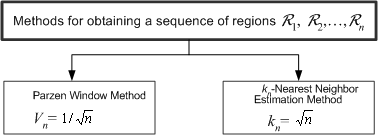
\includegraphics[width=7cm]{./images/non-parametric_methods_1.png}
  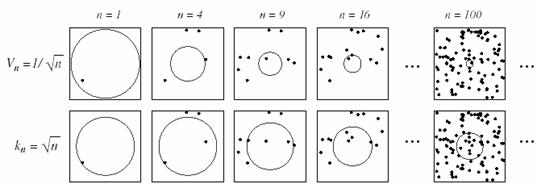
\includegraphics[width=7cm]{./images/non-parametric_methods_2.jpg}
  
  \skriptsubsection{Parzen Windows}{164}
  	The goal of the Parzen Windows method is to estimate a class-conditional probabilty density function $p(\bm x | \omega)$. 
    For this a window function with a defined region $\mathcal{R}_n$ is convoluted with each training sample give class. 
    The sum of all functions gives the density function.\\
    The window function could be, for example, a $d$-dimensional hypercube with $h_n$ being the length of an edge or any other function 
    (Gauss, triangle (Dreieck), \ldots). 
    Often a window with infinite length such as the Gauss window is used, because then the probability will never be zero and a better comparison can be made.\\
    \begin{minipage}{13cm}
    	$$\varphi_{hypercube}(\bm{u}) = \begin{cases}
	    1 &|u_j| \leq 1/2 \quad  j=1,\ldots,d\\
	    0 & \text{otherwise}
	    \end{cases}$$
	    Therefore, the probability can be estimated with
	    $$p(\bm{x}|\omega_j) = \frac1{n_j} \sum_{i=1}^{n_j} \frac{1}{V_{n_j}} \varphi \left(\frac{\bm{x}-\bm{x}_i}{h_{n_j}} \right) \quad 
	    \text{with the conditions } \varphi(\bm{x}) \geq 0 \text{ and } \int \varphi(\bm{u}) du = 1 $$
	    $n_j$ is the number of training sample given class $j$. \\
    \end{minipage}
    \begin{minipage}{5cm}
        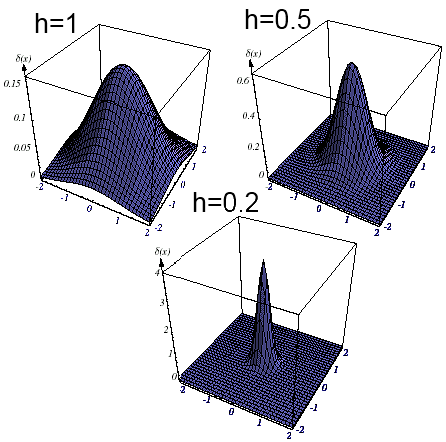
\includegraphics[width=4cm]{./images/parzenWindow.png}
    \end{minipage}
    
    Choosing $h_n$ is important! If $h_n$ (which leads to $V_n$) is too large, the resolution of the
    estimate is too small; if $h_n$ is too small, the statistical variability is too high.
    
  
  \skriptsubsubsection{Probabilistic Neural Networks}{172}
  A PNN is a Parzen window with a Gaussian window function where all data has to be normalized.\\
    \begin{tabular}{ll}
      \parbox{7cm}{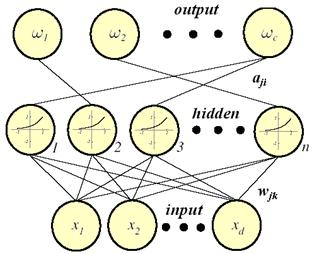
\includegraphics[width=5.5cm]{./images/probabilistic_neural_network.jpg}}
      & \parbox{11cm}{
      Legend:
      \begin{liste}
        \item $d$ input units
        \item $n$ pattern units (one per training sample)
        \item $d$ dimensions
        \item $c$ categories ($\omega_i, i=1,\ldots,c$)
        \item Connections from input to pattern units are modifiable weights, which are trained.
        Now $\bm{w}$ is used instead of $\bm{\theta}$.
        \item \hilight{All (training and input) data must be normalized}: $\sum\limits_{i=1}^d x_i^2 = 1$
      \end{liste}}
    \end{tabular}
    
    \subsubsubsection{Training} is quite easy. Add a new hidden node, set $\bm{w}_k = \frac{\bm{x}_k}{\sqrt{||x||^2}}$ for all training samples 
    and connect every node to the specific category $\omega_k$.
    
    \subsubsubsection{Classification} uses an activation function 
    $\varphi\Big(\frac{\bm{x}-\bm{w}_k}{h_n}\Big) = e^{\frac{\bm{w}_k^T \bm{x}-1}{\sigma^2}}$ 
    with $\sigma$ being a degree of freedom.
    
    PNNs have a high learning speed but need a lot of memory (high space complexity). However,
    speed complexity can be reduced easily by implementing the net activation function evaluation in
    parallel.
    
  
  \skriptsubsection{$k_n$-Nearest-Neighbor Estimation}{174}
    \begin{tabular}{ll}
      \parbox{7cm}{
        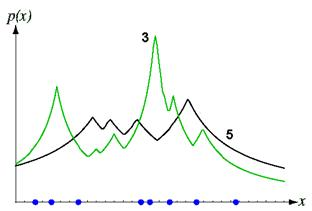
\includegraphics[width=6cm]{./images/k-nearest-neighbor.jpg}
          }
        & \parbox{11cm}{
          Instead of searching the best window function, it can also be adjusted to the training data 
          (also called \em prototypes\em).
          
          Regarding the probability function $p_n(\bm{x}) = \frac{k_n/n}{V_n}$, $k_n$ and $n$
          and therefore $k_n/n$ are fixed and only the volume is adjusted. $k_n$ is now the degree 
          of freedom and good value can be $k_n = \sqrt{n}$.
          
          The figure shows the training samples on the $x$-axis and two possible probability
          with $k_n=3$ and $k_n=5$. The curve is continuous, but the first derivation (slope) is not. 
          In comparision the $k_n$-Nearest-Neighbor to the Parzen-Window estimation the curve is spikier, especially when a Gaussian window is used 
          in the Parzen window method.
          }
    \end{tabular} 
    \vspace{3mm}\\
    Instead of estimate the probability density and calculate the \textbf{a posteriori probabilities} $\bm {P(\omega_i | \bm x)}$ with Bayes, the a posteriori 
    probabilities can be directly calculated out of the training data:\\
    $$ P_n(\omega_i|\bm x)=\frac{k_i}{k}$$
    where $k_i$ is the number of training sample of class $\omega_i$ within a volume $V$ around $\bm x$.
    $k$ is the total number of training samples also within the volume $V$.
  
  
  \skriptsubsection{Nearest-Neighbor Rule}{177}
  	The nearest-neighbor is a simplification of $k_n$-nearest-neighbors, in particular $k=1$. 
  	The class the given test sample will be the same class as the ``next'' trainings sample.
  	
  	\skriptsubsubsection{Convergence of the Nearest Neighbor}{181}
    The error rate of the nearest-neighbor rule is not optimal, it is usually worse than the Bayes 
    rate (minimum). However, it is never worse than twice the Bayes rate. 
    In the best case, if the a-posteriori probabilities of all classes are the same
    the error rate is the same as the Bayes error rate ($\frac{c-1}{c}$).\qquad Error bound: $P^*\leq P\leq P^*\left(2-\frac{c}{c-1}P^*\right)\approx 2P^*$ \\

  \begin{minipage}{14.5cm}
		\skriptsubsection{$k$-Nearest-Neighbor Rule}{182}
		The classifier assigns the label $\omega_m$ to the input of the highest number of samples among the $k$
		nearest samples. Therefore, $k$ shouldn't be a multiple of the number of classes $c$. 
		The error rate is better than with Nearest-Neighbor. If $k=\infty$
		the error rate will be the same as the Bayes error rate. 
		
		This can also be seen as an estimate of the a posteriori probabilities $P(\omega_i|\bm x)$.
		
		\skriptsubsection{Computational Complexity}{184}
  \end{minipage}
  \hfill
  \begin{minipage}{4cm}
	  	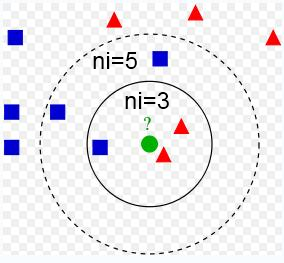
\includegraphics[width=4cm]{./images/kNearest.png}
  \end{minipage}
  
    High complexity in space and time especially when having a lot of features (dimensionality)!
    Reduce by: 
    \begin{aufzaehlung}
    	\item Use the square distance instead of the use the square route to compare: $D_r(a,b)=\sum\limits_{k=1}^r(a_k-b_k)^2$ 
    	instead of  $D_r(a,b)=\left(\sum\limits_{k=1}^r(a_k-b_k)^2\right)^{1/2}$
    	\item Calculate partial distances during classification (abort calculating the distance if it 
    	is already higher than the $k$-nearest ones)
    	\item Eliminate unused prototypes (pruning) by algorithm 3, p.186. This has the disadvanture that a new traning sample can't be easily added.
    	\item Form a search tree during training: Divide search field into subfields (e.g. 2D: 
    	1 search field leads to 4 quadrants). It's much faster, but does not necessarily yield to the best solution.
    \end{aufzaehlung}
  
  \skriptsubsection{Metrics}{187}
    A metric gives a generalized scalar distance between different arguments (vectors, functions, etc.). 
    The metrics has  a big influence in the Nearest-Neighbor. \textbf{Scaling!!!}
  
    
    \subsubsection{Properties}
    \begin{tabular}{llll}
      Nonnegativity: &$D(\bm a, \bm b) \geq 0$ &
      Reflexivity:   &$D(\bm a, \bm b) = 0 \text{ if } \bm a = \bm b$\\
      Symmetry:      &$D(\bm a, \bm b)=D(\bm b, \bm a)$ &
      Triangle inequality: & $D(\bm a, \bm b) + D(\bm b, \bm c) \geq D(\bm a, \bm c)$
    \end{tabular}
    
    \subsubsection{Euclidean Distance / L2-Norm / Pythagoras}
      Definition: $D(\bm a, \bm b) = \sqrt{\sum\limits_{k=1}^d (a_k - b_k)^2}$
      
      Problem of Euclidean distance (``Pythagoras''): When scaling the axes, the metric changes (e.g. 
      axis $x_1$ is measured in $mm$ and axis $x_2$ in $cm$, the distance is not consistent).
      
      
    \subsubsection{Manhattan Metric / L1-Norm / City Block Distance}
      Shortest path between $\bm a$ and $\bm b$ following the coordinate axis.
    
    \subsubsection{Minkowski Metric / Lk-Norm}
    \subsubsection{Tanimoto Metric}
    
    \subsubsection{Selection of a Metric}
      Hard to choose, usually selection is dictated by computational concerns not to prior knowledge
      about the distributions.
      
